\documentclass[11pt, a4paper]{article}

\usepackage[a4paper, top=2.2cm, bottom=2.2cm, left=2.2cm, right=2.2cm]{geometry}
\usepackage{fontspec}

\usepackage[english, bidi=basic, provide=*]{babel}

\babelprovide[import, onchar=ids fonts]{english}
\babelprovide[import, onchar=ids fonts]{italian}

\babelfont{rm}{Noto Sans}

\usepackage{enumitem}
\setlist[itemize]{label=\textcolor{primary}{\textbullet}, leftmargin=*, itemsep=2pt, parsep=0pt}

% --- CUSTOM STYLING PACKAGES ---
\usepackage{xcolor}
\usepackage{titlesec}
\usepackage{tabularx}
\usepackage{parskip}
\usepackage{graphicx}

\definecolor{primary}{HTML}{1A4B84}
\definecolor{textdark}{HTML}{222222} 

\color{textdark}

\titleformat{\section}
  {\Large\bfseries\color{primary}} 
  {}
  {0em} 
  {}
  [\vspace{-0.3em}\textcolor{primary}{\rule{\textwidth}{1pt}}] 
\titlespacing*{\section}{0pt}{3.5ex}{1.5ex}

% Macro personalizzata per le voci di Esperienza e Istruzione
\newcommand{\resumeItem}[4]{
  \vspace{1.5mm}
  \noindent
  \begin{tabular*}{\textwidth}{@{}l@{\extracolsep{\fill}}r@{}}
    \textbf{#1} & \textbf{\textcolor{primary}{#2}} \\
    \textit{#3} & \textit{#4} \\
  \end{tabular*}
  \vspace{1mm}
}

% Hyperref (DEVE ESSERE L'ULTIMO)
\usepackage[colorlinks=true, urlcolor=primary, linkcolor=primary]{hyperref}

\begin{document}

% --- INTESTAZIONE CON SEGNAPOSTO FOTO ---
\noindent
\begin{minipage}[c]{0.75\textwidth}
    {\Huge \textbf{\textcolor{primary}{GIACOMO LOMBARDO}}}\\[0.5em]
    {\Large \textbf{Computer Engineer $|$ AI and Deep Learning Focus}}\\[1em]
    \small
    \href{mailto:giacomolombardo67@gmail.com}{giacomolombardo67@gmail.com} \quad|\quad 
    +39 3248703757 \\[0.3em]
    Santa Ninfa (TP) / Palermo - Italy \\[0.3em]
    \href{https://www.linkedin.com/in/giacomo-lombardo-a944b8315/}{linkedin.com/in/giacomo-lombardo-a944b8315} \\
    \href{https://github.com/Giacomo0303}{github.com/Giacomo0303}
\end{minipage}%
\begin{minipage}[c]{0.25\textwidth}
    \begin{flushright}
        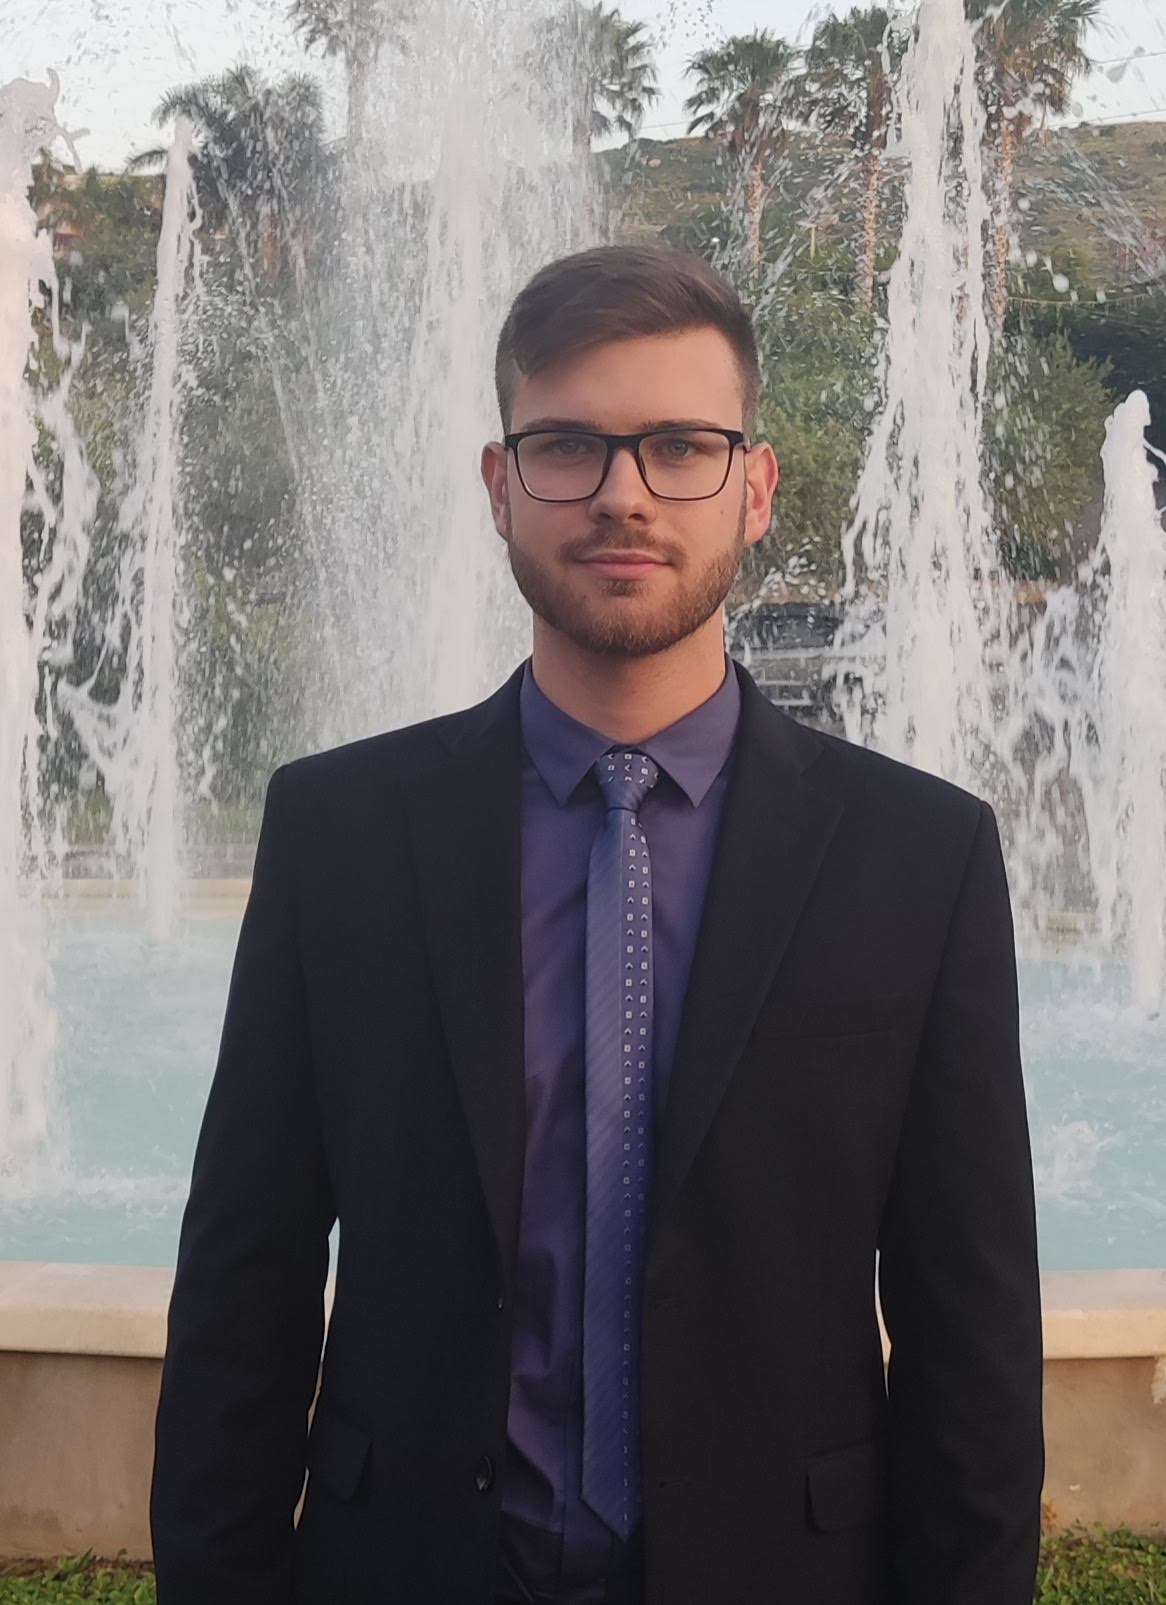
\includegraphics[width=3.5cm]{img.jpg}
    \end{flushright}
\end{minipage}
\vspace{1.5em}

% --- PROFILO ---
\section{Professional Profile}
Computer Engineer pursuing a Master's Degree (expected graduation July 2026), specializing in \textbf{Artificial Intelligence}. Driven by a strong commitment to continuous learning, problem-solving, and analytical thinking, I have extensive experience in teamwork, having completed most of my academic projects in groups of up to five people. Throughout my academic career, I have developed a deep understanding of \textbf{Machine Learning} and \textbf{AI} techniques, focusing primarily on \textbf{Computer Vision} and \textbf{NLP}. I am proficient in frameworks such as PyTorch and TensorFlow, a skill set further refined through various academic projects and my Master's thesis, which focuses on the optimization of Vision Transformers using Pruning and Neural Architecture Search (NAS). I am highly motivated to contribute to the development of innovative AI/ML solutions within a stimulating professional environment.

% --- COMPETENZE ---
\section{Technical Skills}
\begin{itemize}
    \item \textbf{Artificial Intelligence:} Computer Vision, Natural Language Processing (NLP), Deep Learning, Machine Learning.
    \item \textbf{AI Frameworks and Libraries:} PyTorch, TensorFlow, Keras, Scikit-learn, Pandas, NumPy.
    \item \textbf{Programming Languages:} Python (Focus on AI \& Data Science), Java, C, JavaScript.
    \item \textbf{Databases, Data, and Systems:} Graph Databases (Neo4j), Relational Databases (SQL), JSON, XML, Linux, Windows.
    \item \textbf{Tools and IDEs:} PyCharm, Visual Studio Code, Git.
\end{itemize}

% --- PROGETTI ---
\section{Relevant Projects}
\begin{itemize}
    \item \textbf{ViT Compression Framework} $|$ \textit{PyTorch} \\
    Design and development of a framework for the compression of Vision Transformer models. Optimization of computational efficiency through Neural Architecture Search (NAS) and pruning techniques.

    \item \textbf{DeepFake Detection with Attention} $|$ \textit{TensorFlow, Keras} \\
    Development of a system for deepfake image recognition. Initially implemented using classical ML models, then through standard CNN architectures and CNNs equipped with \textbf{Attention} mechanisms.

    \item \textbf{SVD CNN Optimization} $|$ \textit{MATLAB} \\
    Mathematical analysis and implementation of Singular Value Decomposition (SVD) to evaluate the effects of dataset compression on the classification performance of a Convolutional Neural Network.

    \item \textbf{Face Morphing} $|$ \textit{Python, OpenCV} \\
    Computer Vision system for the automatic generation of smooth video transitions (morphing) between faces starting from two static input images.

    \item \textbf{Software Engineering and Full-Stack Development} $|$ \textit{Java, Spring Boot, Kotlin, SQL} \\
    Development of several end-to-end software applications, including a sports management system with UML documentation (Java/MySQL), a workshop management platform with a Spring Boot back-end and jQuery front-end, and a native Android app in Kotlin.
\end{itemize}

% --- ESPERIENZA ---
\section{Professional Experience}

\resumeItem{AI Developer / Intern}{July 2023 -- October 2023}{ITALTEL S.p.A.}{Carini (PA)}
Curricular Internship.
\begin{itemize}
    \item \textbf{Main Project:} Design and development of Computer Vision software dedicated to the automatic recognition and counting of labels in photographic inputs.
    \item \textbf{Stack and Skills:} Development and training of Machine Learning models using \textbf{TensorFlow} and \textbf{Keras} APIs.
    \item \textbf{Architectures:} Design, implementation, and training of \textbf{Convolutional Neural Networks (CNN)} for image analysis and classification.
\end{itemize}

% --- ISTRUZIONE ---
\section{Education and Training}

\resumeItem{Master's Degree in Computer Engineering (LM-32)}{2024 -- Ongoing}{University of Palermo}{Palermo}
\vspace{-1.5em}
\begin{itemize}
    \item Thesis based on Transformer model compression through pruning and architectural search techniques.
\end{itemize}

\resumeItem{Bachelor's Degree in Computer Engineering (L-8)}{2021 -- July 2024}{University of Palermo}{Palermo}
\vspace{-1.5em}
\begin{itemize}
    \item Final grade: \textbf{110/110 cum laude}
\end{itemize}

\resumeItem{High School Diploma (Applied Sciences)}{2016 -- 2021}{Michele Cipolla Scientific High School}{Castelvetrano (TP)}
\vspace{-1.5em}
\begin{itemize}
    \item Final grade: \textbf{100/100 cum laude}
\end{itemize}

% --- CERTIFICAZIONI E LINGUE ---
\section{Certifications and Languages}
\begin{itemize}
    \item \textbf{English:} B2 Level.
    \item \textbf{Italian:} Native Speaker.
\end{itemize}

\vfill
\begin{center}
\scriptsize{\textit{I hereby authorize the processing of my personal data in accordance with Legislative Decree June 30, 2003, n. 196 and the GDPR (EU Regulation 2016/679).}}
\end{center}

\end{document}